%%% -*-LaTeX-*-

\chapter{SweetPea Overview}

SweetPea is a software system for creating replicable, statistically robust experimental designs. SweetPea consists of a high-level language and a runtime. The language provides primitives that closely match the terms that scientists use to describe their experimental designs. The runtime synthesizes an experimental sequence which is guaranteed to not prefer any valid solution over any other. SweetPea provides this guarantee by representing the experiment as a boolean formula and interfacing with a SAT sampler; this constrains the high-language to be amenable to being translated into a boolean formula.

The ultimate vision for SweetPea is for the researcher to declaratively describe the analysis they wish to perform, and for the system to automatically derive the constraints required to produce an experiment for the desired analysis. Further, the sytems would ideally interactively iterate with the user to let them explore exactly what they wanted to analyze, and how choices they make effect the feasibility of the experimental design.

In this chapter we'll identify the fundamental components of an experimental design by looking at simple version of a classic psychology experiment, the Stroop test. Then we'll see how these components are represented in the language and the goals of the runtime.

\section{Running Example: the Stroop Experiment}

The Stroop experiment is a well-known psychology experiment, originally published by John Stroop in 1935. A subject is shown a stimulus, and asked to perform a task based on some property of the stimulus; the researcher measures how the subject's reaction time varies depending on the stimulus. One version of this experiemnt involves showing subjects a word printed on a slide and asking them to say the color of the word. All of the words are the names of colors, such as the text 'red' and 'blue'. Some of the stimuli are congruent, meaning that the color of the ink matches the text, such as the word red printed in red ink. Other stimuli are incongruent, such as the word red printed in blue ink (figure \figref{stroop_example}). The Stroop effect is the observation that subjects have a longer reaction time when the stimulus is incongruent.

Let's consider the smallest version of the Stroop experiment, where the stimuli consist of two colors. Each stimulus is specified by independent and control variables, called \emph{factors}: ink color and text. Each factor has two \emph{levels}, red and blue. Figure \figref{simple_full_crossing} shows the \emph{full crossing} of these factors for this simple case, for a total of 4 possible stimuli. For reference, real experiments have on the order of 5 to 8 factors with 2 to 4 levels, leading to tens to hundreds of possible stimuli. The \emph{design} of the experiment is the list of all factors that describe each stimulus. The design of the experiment may contain factors that are not present in the full-crossing.

Each subject is shown an ordering of the possible stimuli. The researchers may want to place additional \emph{constraints} on the ordering, such as first familiarizing the subject with the task by showing some number of congruent stimuli before showing them a mix of congruent and incongruent stimuli. For our small example, let's consider the constraint that there should be no repetitions of stimuli whose text is the same. The ordering in \figref{simple_full_crossing} is a valid ordering which satisifies these constraints, but swapping the order of the first and second trial would produce an invalid ordering under those constraints.

To prove that we do not introduce bias because of the way we construct experimental sequences, we would like to ensure that each valid sequence is equally likely. In this example, we have four stimuli so there are 4 factorial = 24 possible orderings. Of those 24 orderings, 8 satisfy the constraints as shown in \figref{valid_seqs}, and to provide this guarantee we want each of those 8 to be equally likely.


\begin{figure}[t]%
    \centering
    \subfloat[A congruent Stroop stimulus.]{{
\includegraphics[width=7cm]{fig_red_in_red} }}%
  %  \qquad
    \subfloat[An incongruent Stroop stimulus.]{{
\includegraphics[width=7cm]{fig_red_in_blue} }}%
    \caption{Example Stroop stimuli.}%
    \label{fig:stroop_example}%
\end{figure}


\begin{figure}[t]%
    \centering
    \subfloat[The full crossing of possible stimuli.]{{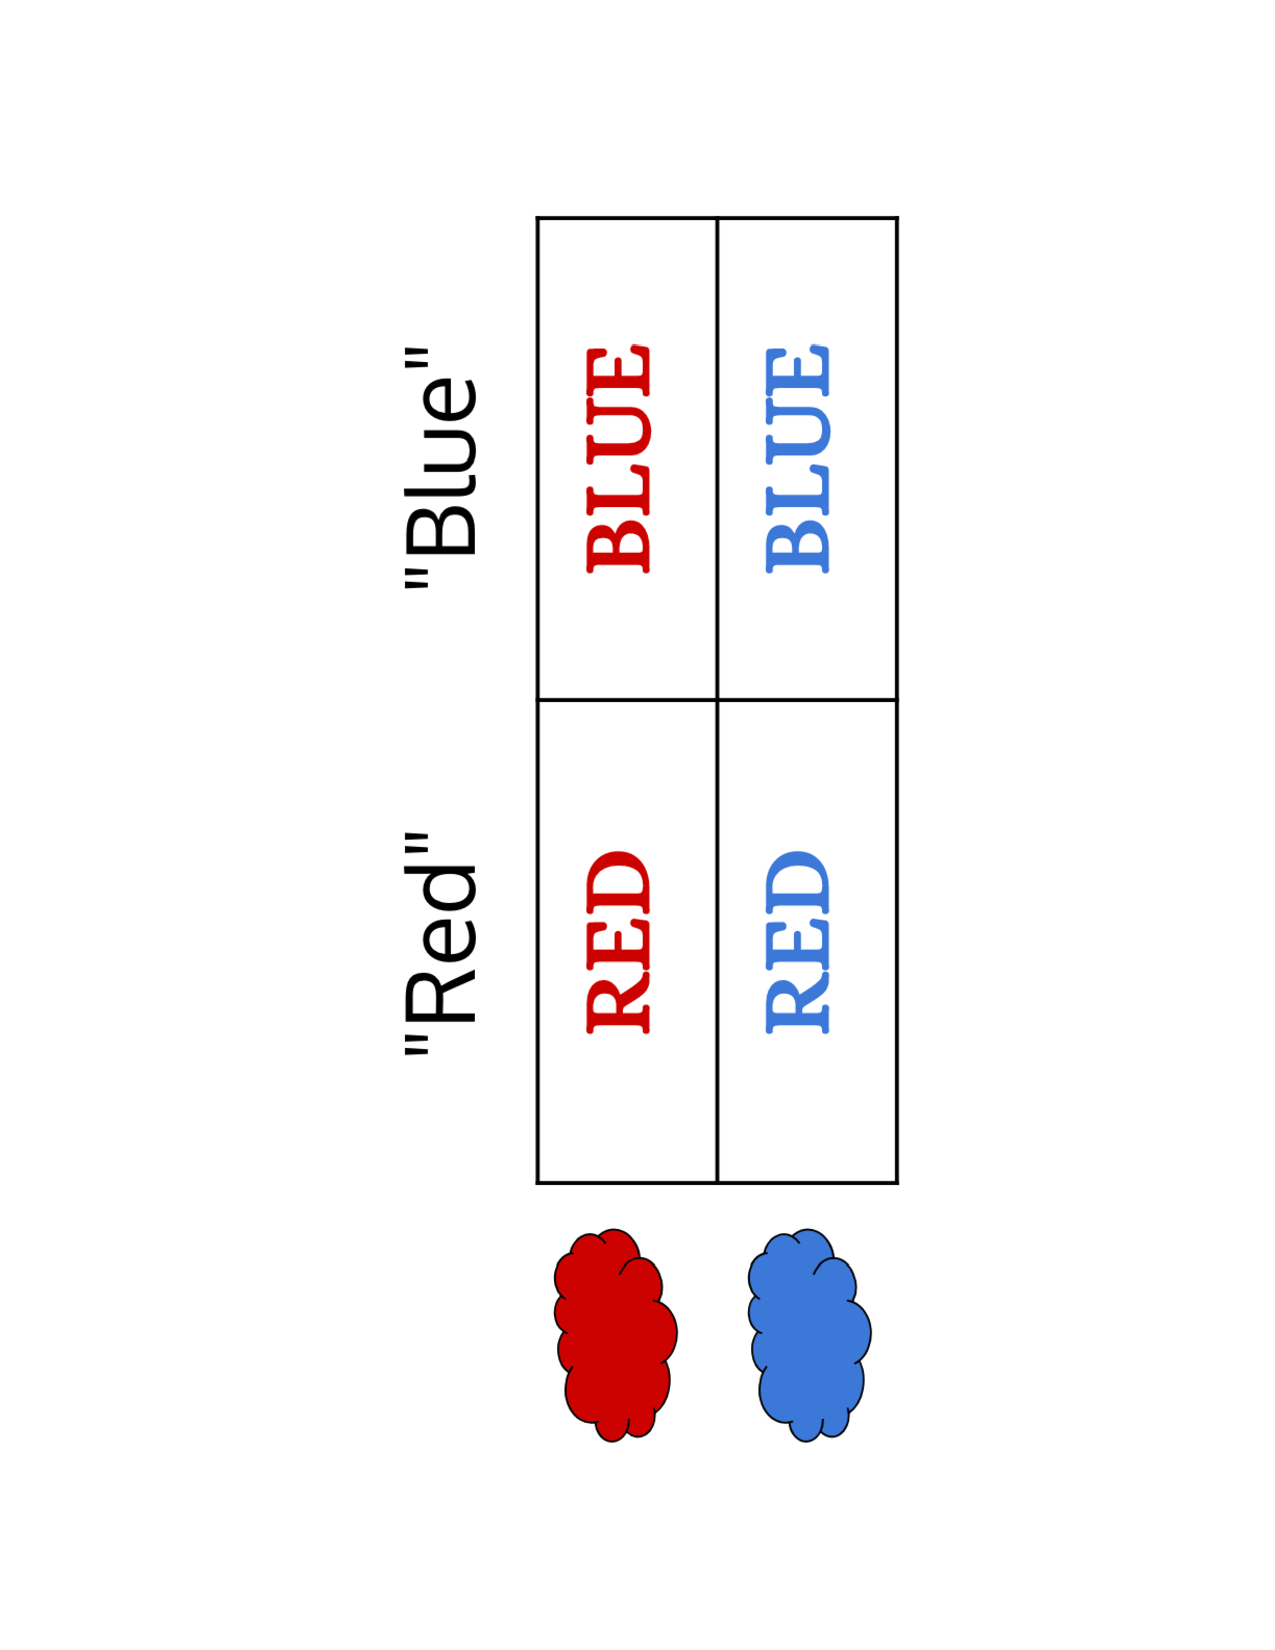
\includegraphics[angle=270,origin=c,width=8cm]{fig_simple_full_crossing}}}%
  %  \qquad
    \subfloat[A possible ordering of stimuli.]{{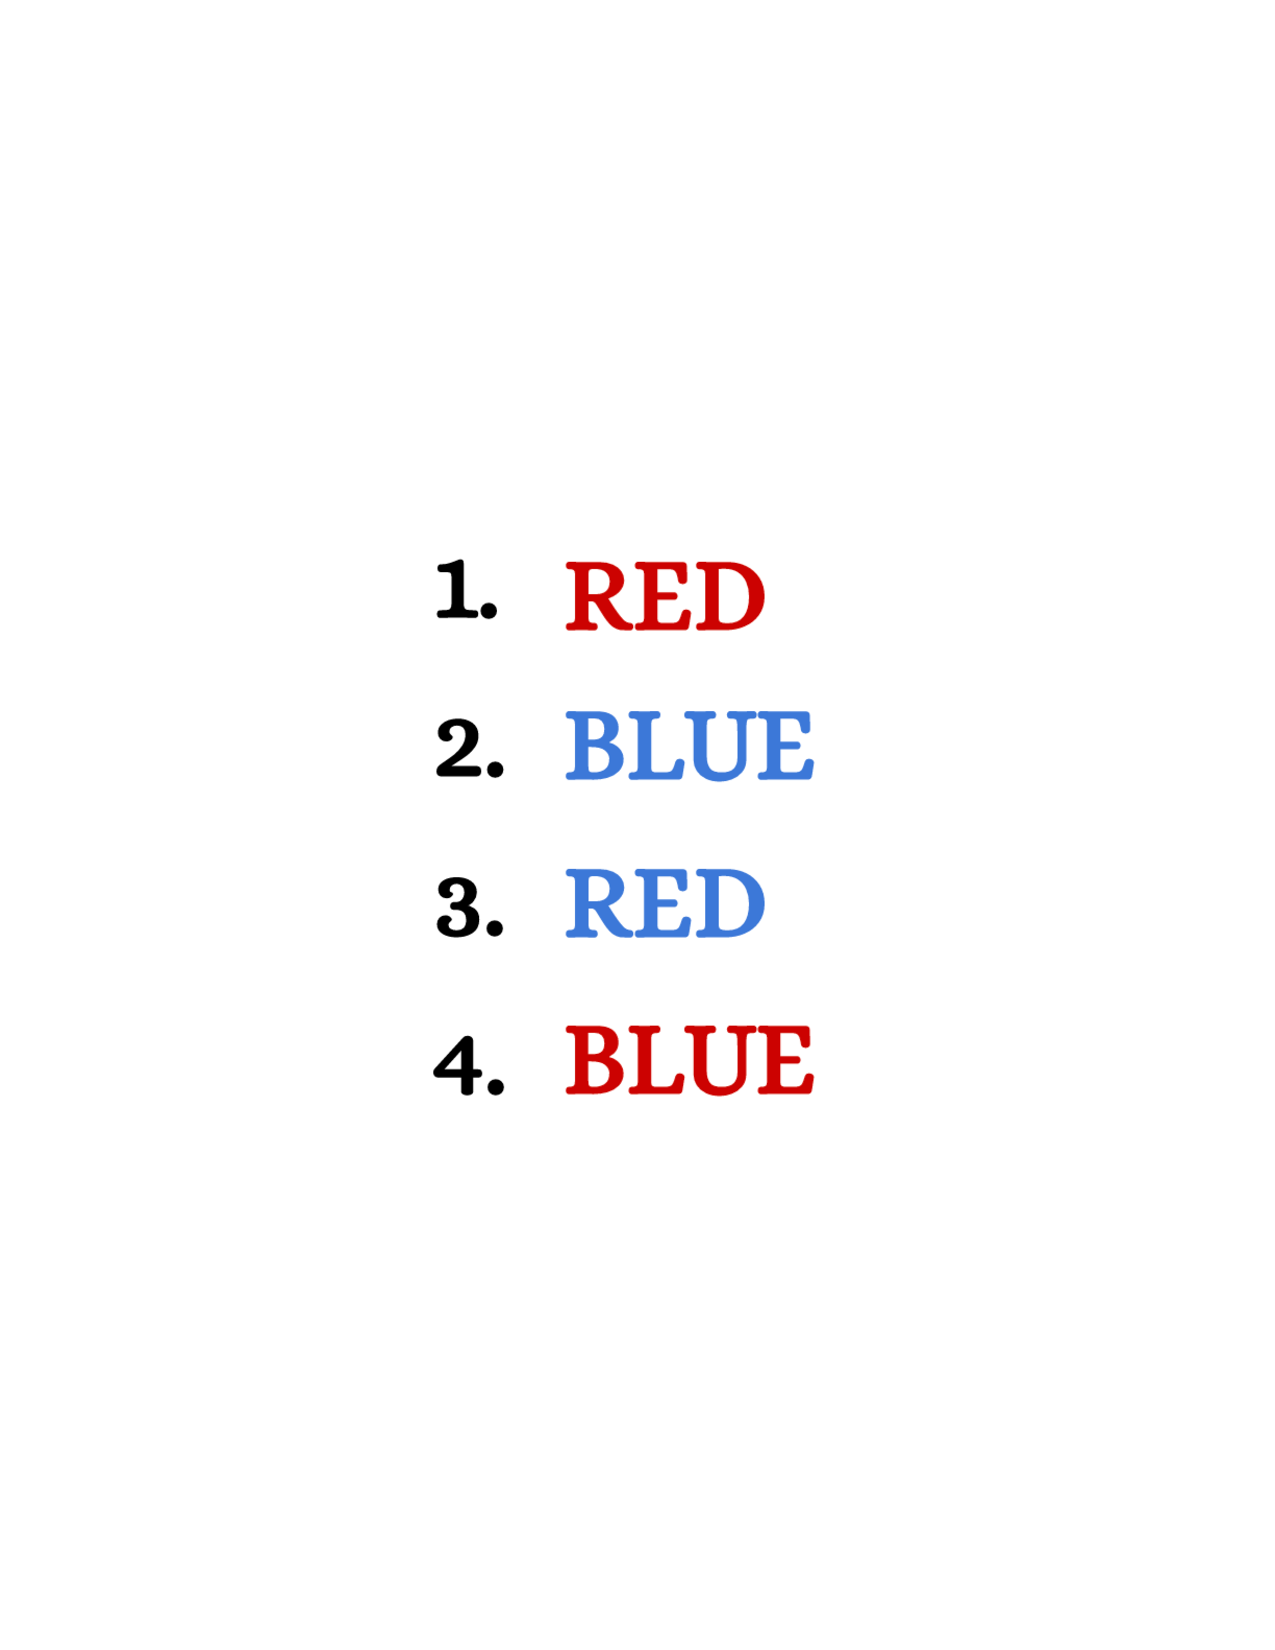
\includegraphics[width=7cm]{fig_possible_ord} }}%
    \caption{All stimuli and a possible ordering.}%
    \label{fig:simple_full_crossing}%
\end{figure}



\begin{figure}[t]
    \centerline{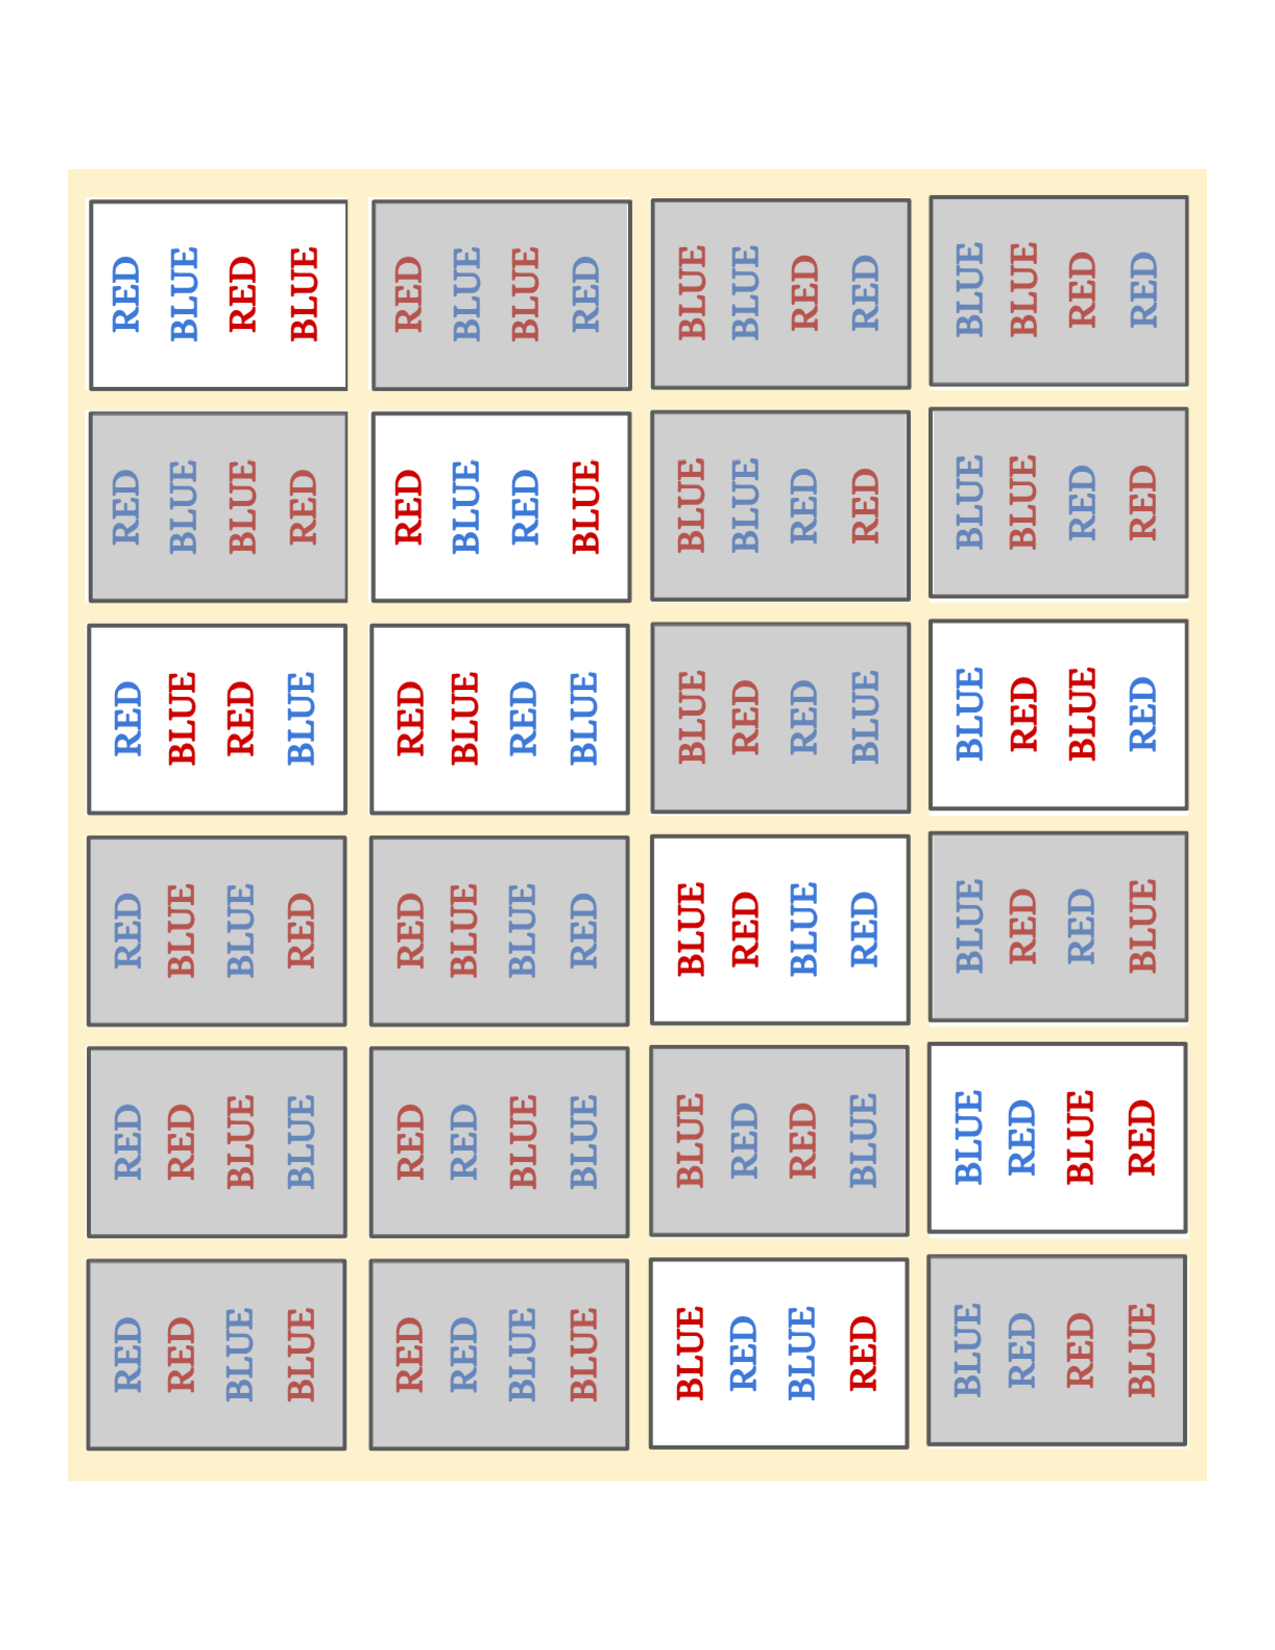
\includegraphics[angle=270,origin=c,width=10cm]{fig_valid_seqs}}
    \caption{Of the 24 possible orderings, the highlighted 8 satisfy the constraints.}%
    \label{fig:valid_seqs}%
\end{figure}


\section{A Language for Experimental Design}

Let's see how the simple Stroop experiment can be represented in SweetPea, and then at how that representation can be translated to a boolean formula to generate an experimental sequence.

The version of the SweetPea language we'll discuss is embedded in Python, so uses Python syntax.

First, we represent the factors directly as a list of levels:

%\begin{code}
\begin{verbatim}
ink_color = ("ink_color", ["red", "blue"])
text      = ("text",      ["red", "blue"])
\end{verbatim}
%\end{code}

Next, let's represent the constraint that there should be no repetitions of stimuli whose text is the same. \begin{verbatim} NoMoreThanKInARow \end{verbatim} is a constraint constructor function in SweetPea, which allows us to declaratively specify the constraint:

\begin{verbatim}
k = 2
constraints = [NoMoreThanKInARow(k, ("text", "red")),
               NoMoreThanKInARow(k, ("text", "blue"))]
\end{verbatim}

Having specified the factors and the constraints over those factors, we can now specify the rest of the experimental design:

\begin{verbatim}
design = [ink_color, text]
crossing = design

experiment = full_crossing(design, crossing, constraints)

synthesize_trials(experiment)
\end{verbatim}

In this example, the design and the full crossing are the same, though that doesn't need to always be the case. We specify the experiment to be the full crossing, but more generally we can construct experiments out of multiple "blocks" of crossings. The call to synthesize\_trials translates the experiment to a boolean formula representation and calls the SAT sampler.

\section{A Runtime for Uniform Sampling}

A \emph{boolean formula} consists of \emph{boolean variables} combined using boolean operators, such as AND, OR and NOT. A \emph{satisfying assignment} is a specification of True or False to each boolean variable which causes the entire formula to evaluate to True. Some formulas are unsatisfiable.

An example of an unsatisfiable formula is (A AND (NOT A)). Regardless of whether A is True of False, this formula will always evaluate to False. In contrast, the formula (A AND B) is satisfied by the assignment A is True and B is True, because (True AND True) evaluates to True.

How do we represent the program above as a boolean formula?

First, we represent each level of each trial as a boolean variable, which corresponds to whether or not that level is chosen for the produced experimental sequence. For our Stroop example, there are 4 trials, each of which have 4 boolean variables corresponding to each of the levels for a total of 16 boolean variables. A real experiment will have on the order of hundreds to thousands of boolean variables. These level variables are bound by additional constraints such as that only one level per factor is true, as well as constraints that say how many instances of a level should exist in a given experimental block.

For our Stroop example, this means that for each trial we create boolean variables to represent ink\_color=red, ink\_color=blue, text=red, text=blue. We create boolean formulas for each trial which say that exactly one of ink\_color=red or ink\_color=blue must be true, and that there must be two ink\_color=red's in the fully crossed block.

We have multiple strategies for encoding constraints, but for now let's say we have a strategy for encoding constraints of the form "no more than K in a row". We can use this to encode our constraint that there should be no repetitions of stimuli whose text is the same.

Once we've created this boolean formula which represents all the relationships which the levels must fulfill, we can pass this formula to the SAT sampler. If there exists an assignment of the boolean variables which satisfies all the constraints, the sampler will return one such assignment. If there are no satisfying assignments the sampler will state that the formula is unsatisfiable.

The solution that the sampler finds is guaranteed to be approximately uniformly probable in the space of all possible solutions. We currently use the SAT sampler Unigen which uses universal hash functions to find solutions in a principled way, but providing this guarantee is the goal of all uniform sampling. Unigen guarantees that it will return a satisfying assignment with approximately uniform probability of choosing any satisfying assignment to a given boolean formula.

How does this guarantee, which is provided at the level of boolean variables, translate to the guarantee we want, at the level of the experimental design? As we'll discuss further in Chapter 4, so long as every boolean formula uniquely describes a single experimental design, we know that the satisfying experiemental sequence is approximately uniformly probable among all satisfying experimental sequences. For our Stroop example, this means that each of the 8 valid orderings in \figref{valid_seqs} should be approximately equally likely.

If the sampler finds a satisfying assignment to the variables, we can then translate those variables back to the levels they represent. For our Stroop example, this means we will get assignments to the 16 boolean variables, 4 of them for each trial. These will determine the values of each of the trials, and because we have satisfied all the necessary constraints, results in a valid ordering of the trials.

We'll revisit this example in Chapter 7 to see an end-to-end encoding of the Stroop experiment, as well as the sequences produced by SweetPea.
